\cellname{LEFTBUF}
\designer{Henry Lovett}
\celldescription{A start of row buffer cell.}

This cell is to be placed at the beginning of each row of cells. 
The purpose of this cell is to buffer the \textit{Clock, nReset} and \textit{Test} signals to attempt to eliminate skew of the signals.
They also cater for the scan path in the circuit by routing and buffering the signal.

This cell contains 3 large buffers, each made up of 4 stages.
The gain of the stages are gradually increased, relative to the first. 
The transistors were folded to reduce the vertical height of the cell. 
The total, and folded sizes of the transistors are seen in the table below.

\begin{table}[htb!]
\centering
\begin{tabular}{c|cccc}
Stage						&	1				&	2		&	3		&	4 \\ \hline
Gain 						& 	1 				& 	2.7 	& 	7.3 	& 	20 \\
$W_n$ unfolded 	($\mu m$) 	&	1.0 			& 	2.7 	& 	7.3 	& 	20 \\
$W_p$ unfolded	($\mu m$)	& 	2.9				& 	7.85 	& 	21.2 	& 	58 \\
$W_n$ folded	($\mu m$)	&	$1 \times 1.0$ 	& 	$1 \times 2.7$ 		& 	$1 \times 7.3$ 		& 	$2 \times 10.0$ \\
$W_p$ folded	($\mu m$)	&	$1 \times 2.9$ 	& 	$1 \times 7.85$ 	& 	$2 \times 10.6$ 	& 	$4 \times 14.5$ \\
\end{tabular}
\end{table}

\stickdiagram{../leftbuf/stickdiagram.pdf}
\acchar{../leftbuf/acresults.txt}
\transistor{../leftbuf/transistorcd.pdf}

%override of default
\subsubsection*{HSpice Simulation}
\begin{figure}[ht!]
        \centering
        \begin{subfigure}[b]{0.45\textwidth}
                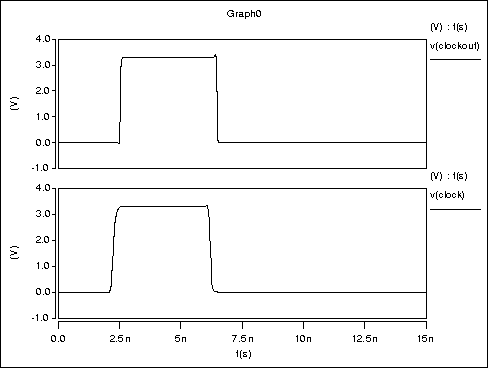
\includegraphics[width=\textwidth]{../leftbuf/hspiceClock.png}
        \end{subfigure}%
        ~ %add desired spacing between images, e. g. ~, \quad, \qquad etc.
          %(or a blank line to force the subfigure onto a new line)
        \begin{subfigure}[b]{0.45\textwidth}
                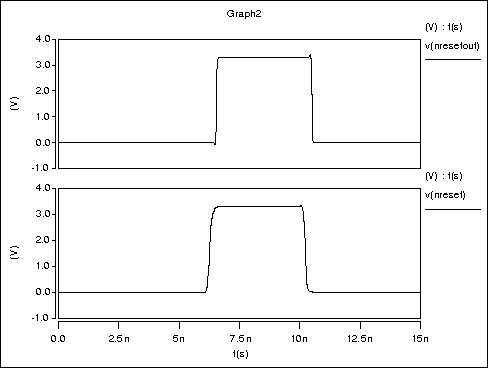
\includegraphics[width=\textwidth]{../leftbuf/hspiceNReset.png}
        \end{subfigure} 
		~ %add desired spacing between images, e. g. ~, \quad, \qquad etc.
          %(or a blank line to force the subfigure onto a new line)
        \begin{subfigure}[b]{0.45\textwidth}
                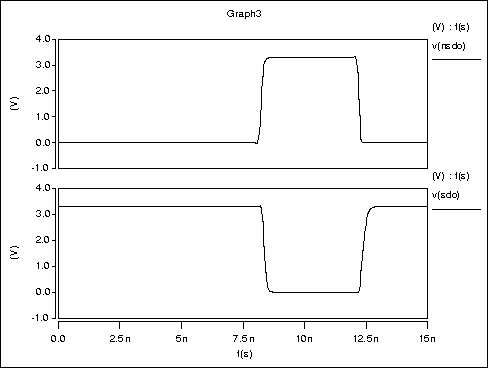
\includegraphics[width=\textwidth]{../leftbuf/hspiceSDO.png}
        \end{subfigure} 
		~ %add desired spacing between images, e. g. ~, \quad, \qquad etc.
          %(or a blank line to force the subfigure onto a new line)
        \begin{subfigure}[b]{0.45\textwidth}
                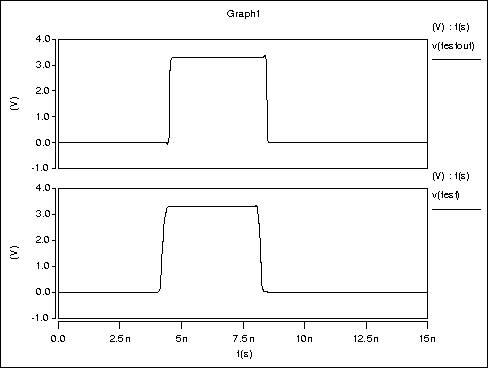
\includegraphics[width=\textwidth]{../leftbuf/hspiceTest.png}
        \end{subfigure}
\end{figure}
